\documentclass{article}
\usepackage{amsmath, amssymb}
\usepackage{graphicx}
\usepackage{float}
\usepackage[margin=1in]{geometry}
\usepackage{caption}

\begin{document}

\section*{Question 1}

\subsection*{(a) OLS Solution}
We consider the OLS minimization problem
\[
\min_{\beta_0, \beta_1} \sum_{i=1}^n (y_i - \beta_0 - \beta_1 x_i)^2.
\]
The first-order conditions are obtained by setting the derivatives with respect to \(\beta_0\) and \(\beta_1\) to zero:
\[
\frac{\partial}{\partial \beta_0}: \quad -2\sum_{i=1}^n (y_i - \beta_0 - \beta_1 x_i) = 0 
\quad \Longrightarrow \quad \sum_{i=1}^n y_i = n\beta_0 + \beta_1\sum_{i=1}^n x_i,
\]
\[
\frac{\partial}{\partial \beta_1}: \quad -2\sum_{i=1}^n x_i (y_i - \beta_0 - \beta_1 x_i) = 0 
\quad \Longrightarrow \quad \sum_{i=1}^n x_i y_i = \beta_0 \sum_{i=1}^n x_i + \beta_1 \sum_{i=1}^n x_i^2.
\]
Defining
\[
S_x = \sum_{i=1}^n x_i,\quad S_{xx} = \sum_{i=1}^n x_i^2,\quad S_y = \sum_{i=1}^n y_i,\quad S_{xy} = \sum_{i=1}^n x_i y_i,
\]
the normal equations become
\[
\begin{cases}
n \beta_0 + S_x \beta_1 = S_y, \\
S_x \beta_0 + S_{xx} \beta_1 = S_{xy}.
\end{cases}
\]
Solving these, we obtain the OLS estimates:
\[
\boxed{\hat{\beta}_1 = \frac{n S_{xy} - S_x S_y}{n S_{xx} - S_x^2}, \quad \hat{\beta}_0 = \frac{S_y S_{xx} - S_x S_{xy}}{n S_{xx} - S_x^2}},
\]
or, equivalently, in terms of sample means \(\bar{x}\) and \(\bar{y}\):
\[
\boxed{\hat{\beta}_1 = \frac{\sum_{i=1}^n (x_i-\bar{x})(y_i-\bar{y})}{\sum_{i=1}^n (x_i-\bar{x})^2}, \quad \hat{\beta}_0 = \bar{y} - \hat{\beta}_1 \bar{x}}.
\]

\subsection*{(b) Lagrangian Formulation}
For the ridge regression problem
\[
\min_{\beta_0, \beta_1} \sum_{i=1}^n (y_i - \beta_0 - \beta_1 x_i)^2 \quad \text{subject to} \quad \beta_0^2 + \beta_1^2 \le t,
\]
we form the Lagrangian function:
\[
\mathcal{L}(\beta_0, \beta_1, \lambda) = \sum_{i=1}^n (y_i - \beta_0 - \beta_1 x_i)^2 + \lambda \left(\beta_0^2 + \beta_1^2 - t\right),
\]
with \(\lambda \ge 0\).

\subsection*{(c) Optimality under NDCQ}
Taking the partial derivatives of \(\mathcal{L}\) with respect to \(\beta_0\) and \(\beta_1\) and setting them to zero gives:
\[
\frac{\partial \mathcal{L}}{\partial \beta_0} = -2\sum_{i=1}^n (y_i - \beta_0 - \beta_1 x_i) + 2\lambda \beta_0 = 0,
\]
\[
\frac{\partial \mathcal{L}}{\partial \beta_1} = -2\sum_{i=1}^n x_i (y_i - \beta_0 - \beta_1 x_i) + 2\lambda \beta_1 = 0.
\]
Using the summary statistics, these equations can be rewritten as:
\[
S_y - n\beta_0 - S_x \beta_1 = \lambda \beta_0,
\]
\[
S_{xy} - S_x \beta_0 - S_{xx} \beta_1 = \lambda \beta_1.
\]
Rearranging, we obtain the regularized normal equations:
\[
(n+\lambda)\beta_0 + S_x \beta_1 = S_y,
\]
\[
S_x \beta_0 + (S_{xx}+\lambda)\beta_1 = S_{xy}.
\]
In matrix form, letting
\[
X = \begin{pmatrix} 1 & x_1 \\ 1 & x_2 \\ \vdots & \vdots \\ 1 & x_n \end{pmatrix}, \quad \boldsymbol{\beta} = \begin{pmatrix}\beta_0 \\ \beta_1\end{pmatrix}, \quad \mathbf{y} = \begin{pmatrix} y_1 \\ y_2 \\ \vdots \\ y_n \end{pmatrix},
\]
the solution is given by:
\[
\boxed{\boldsymbol{\beta} = \left( X^T X + \lambda I \right)^{-1} X^T \mathbf{y}},
\]
where \(I\) is the \(2 \times 2\) identity matrix. Explicitly, the solutions are:
\[
\boxed{\beta_0 = \frac{S_y (S_{xx}+\lambda) - S_x S_{xy}}{(n+\lambda)(S_{xx}+\lambda) - S_x^2}},
\]
\[
\boxed{\beta_1 = \frac{(n+\lambda) S_{xy} - S_x S_y}{(n+\lambda)(S_{xx}+\lambda) - S_x^2}}.
\]

\subsection*{(d) Comparison and Interpretation}
\textbf{OLS Estimates:}
\[
\hat{\beta}_0 = \frac{S_y S_{xx} - S_x S_{xy}}{n S_{xx} - S_x^2}, \quad \hat{\beta}_1 = \frac{n S_{xy} - S_x S_y}{n S_{xx} - S_x^2}.
\]

\textbf{Ridge Regression Estimates:}
\[
\beta_0(\lambda) = \frac{S_y (S_{xx}+\lambda) - S_x S_{xy}}{(n+\lambda)(S_{xx}+\lambda) - S_x^2}, \quad \beta_1(\lambda) = \frac{(n+\lambda) S_{xy} - S_x S_y}{(n+\lambda)(S_{xx}+\lambda) - S_x^2}.
\]

When \(\lambda = 0\), the ridge estimates reduce to the OLS estimates. For \(\lambda > 0\), the additional \(\lambda\) in the denominators increases the effective regularization, shrinking the coefficient estimates towards zero. This shrinkage reduces the variance of the estimates, particularly useful in the presence of multicollinearity or limited data, at the cost of introducing some bias.

\section*{Question 2}

\subsection*{(a)}
Since the original problem is to minimize the portfolio variance
\[
V(x,y,z)=x^2+\frac{1}{2}xy+4y^2+2z^2,
\]
we convert it into a maximization problem by maximizing the negative of the objective. That is, we solve
\[
\max_{x,y,z} \; -\left(x^2+\frac{1}{2}xy+4y^2+2z^2\right).
\]

\subsection*{(b)}
The equality constraints are:
\[
x+y+z=1,
\]
and
\[
1\cdot x+10\cdot y+6\cdot z=4.
\]

\subsection*{(c)}
We form the Lagrangian
\[
\mathcal{L}(x,y,z,\lambda,\mu)=x^2+\frac{1}{2}xy+4y^2+2z^2-\lambda(x+y+z-1)-\mu(x+10y+6z-4).
\]
The first-order conditions are:
\[
\frac{\partial \mathcal{L}}{\partial x}=2x+\frac{1}{2}y-\lambda-\mu=0,
\]
\[
\frac{\partial \mathcal{L}}{\partial y}=\frac{1}{2}x+8y-\lambda-10\mu=0,
\]
\[
\frac{\partial \mathcal{L}}{\partial z}=4z-\lambda-6\mu=0.
\]
Together with the constraints
\[
x+y+z=1 \quad \text{and} \quad x+10y+6z=4,
\]
solving this system (through elimination and substitution) yields the optimal allocation
\[
x=\frac{25}{48},\quad y=\frac{29}{192},\quad z=\frac{21}{64}.
\]

\subsection*{(d)}
To reduce the problem to a univariate unconstrained optimization, express \(x\) and \(z\) in terms of \(y\). From the budget constraint
\[
x=1-y-z,
\]
and the return constraint
\[
x+10y+6z=4,
\]
substitute \(x\) to obtain
\[
1-y-z+10y+6z=1+9y+5z=4,
\]
which implies
\[
5z=3-9y \quad \Longrightarrow \quad z=\frac{3-9y}{5}.
\]
Then,
\[
x=1-y-\frac{3-9y}{5}=\frac{2+4y}{5}.
\]
Substitute these into \(V(x,y,z)\) to get
\[
V(y)=\frac{288y^2-87y+22}{25}.
\]
Differentiating and setting the derivative to zero leads to
\[
y=\frac{87}{576}=\frac{29}{192},
\]
and substituting back gives
\[
x=\frac{25}{48},\quad z=\frac{21}{64}.
\]

\subsection*{(e)}
If the required portfolio return increases from 4 to 4.5, the return constraint becomes
\[
x+10y+6z=4.5.
\]
By sensitivity analysis, the change in the optimal variance is approximated by the Lagrange multiplier \(\mu\) associated with the return constraint:
\[
\Delta V\approx \mu\,\Delta R.
\]
At the optimum, we have
\[
\mu=\frac{-x+5y}{6}=\frac{5}{128}.
\]
Thus, for \(\Delta R=0.5\),
\[
\Delta V\approx \frac{5}{128}\times 0.5=\frac{5}{256}\approx 0.0195.
\]

\subsection*{(f)}
If the mean return of the third stock increases from 6 to 6.5, the return constraint becomes
\[
x+10y+6.5z=4.
\]
Denote the change in the coefficient for \(z\) by \(\delta=0.5\). By the envelope theorem, the sensitivity of the optimal variance with respect to \(\delta\) is
\[
\frac{\partial V^*}{\partial \delta}=-\mu z.
\]
At the optimum, with \(z=\frac{21}{64}\) and \(\mu=\frac{5}{128}\), we have
\[
\frac{\partial V^*}{\partial \delta}=-\frac{5}{128}\cdot\frac{21}{64}=-\frac{105}{8192}.
\]
Thus, for \(\delta=0.5\), the change in the minimum variance is approximately
\[
\Delta V\approx -\frac{105}{8192}\times 0.5=-\frac{105}{16384}\approx -0.00641.
\]

\section*{Question 3}

\subsection*{(a)}
In addition to the budget constraint 
\[
x+y+z=1,
\]
we now require the portfolio mean return to be at least 4 and no short-selling is allowed. Thus, the inequality constraints are
\[
x+10y+6z\ge 4,
\]
and
\[
x\ge 0,\quad y\ge 0,\quad z\ge 0.
\]

\subsection*{(b)}
Writing the problem in standard form we have:

\[
\begin{array}{rl}
\text{minimize} & V(x,y,z)=x^2+\frac{1}{2}xy+4y^2+2z^2,\\[1mm]
\text{subject to} & x+y+z=1,\\[1mm]
 & x+10y+6z\ge 4,\\[1mm]
 & x\ge 0,\quad y\ge 0,\quad z\ge 0.
\end{array}
\]

For the inequality constraint \(x+10y+6z\ge 4\), we rewrite it in the form
\[
4-x-10y-6z\le 0.
\]
Let \(\lambda\) be the Lagrange multiplier for the equality constraint, \(\mu\ge 0\) for the inequality \(4-x-10y-6z\le 0\), and \(\alpha,\beta,\gamma\ge 0\) for the non-negativity constraints on \(x\), \(y\), and \(z\) (written as \(-x\le 0\), \(-y\le 0\), \(-z\le 0\), respectively).

Then the Lagrangian is
\[
\mathcal{L}(x,y,z,\lambda,\mu,\alpha,\beta,\gamma)=x^2+\frac{1}{2}xy+4y^2+2z^2-\lambda(x+y+z-1)+\mu(4-x-10y-6z)-\alpha x-\beta y-\gamma z.
\]

The first-order (KKT) conditions are:
\[
\begin{aligned}
\frac{\partial\mathcal{L}}{\partial x}&: \quad 2x+\frac{1}{2}y-\lambda-\mu-\alpha=0,\\[1mm]
\frac{\partial\mathcal{L}}{\partial y}&: \quad \frac{1}{2}x+8y-\lambda-10\mu-\beta=0,\\[1mm]
\frac{\partial\mathcal{L}}{\partial z}&: \quad 4z-\lambda-6\mu-\gamma=0,
\end{aligned}
\]
together with the primal feasibility conditions
\[
\begin{aligned}
x+y+z&=1,\\[1mm]
4-x-10y-6z&\le 0,\\[1mm]
x,y,z&\ge 0,
\end{aligned}
\]
the dual feasibility conditions
\[
\mu\ge 0,\quad \alpha\ge 0,\quad \beta\ge 0,\quad \gamma\ge 0,
\]
and the complementary slackness conditions
\[
\mu\,(4-x-10y-6z)=0,\quad \alpha\,x=0,\quad \beta\,y=0,\quad \gamma\,z=0.
\]

\subsection*{(c) (Bonus)}
Under the assumption that a nondegeneracy constraint qualification (NDCQ) holds, the KKT conditions are both necessary and sufficient for optimality.

Notice that the unconstrained optimum from Question 2 is
\[
x=\frac{25}{48},\quad y=\frac{29}{192},\quad z=\frac{21}{64},
\]
which satisfies
\[
x+y+z=1\quad \text{and} \quad x+10y+6z=4,
\]
with \(x,y,z>0\). Therefore, the mean return constraint is binding and the non-negativity constraints are inactive (i.e., \(\alpha=\beta=\gamma=0\)). In this case, the KKT conditions reduce to the same system solved in Question 2:
\[
\begin{aligned}
2x+\frac{1}{2}y-\lambda-\mu&=0,\\[1mm]
\frac{1}{2}x+8y-\lambda-10\mu&=0,\\[1mm]
4z-\lambda-6\mu&=0,
\end{aligned}
\]
with
\[
x+y+z=1\quad \text{and} \quad x+10y+6z=4,
\]
and the complementary slackness condition \(\mu\,(4-x-10y-6z)=0\) implying that \(\mu>0\) (since \(4-x-10y-6z=0\)).

Thus, the optimal solution remains
\[
\boxed{x=\frac{25}{48},\quad y=\frac{29}{192},\quad z=\frac{21}{64}},
\]
with the corresponding multiplier \(\mu\) as determined previously.

\section*{Question 4}
\subsection*{(a)}
We are given the inequalities
\[
x+2y \le 1,\quad y-2x \ge -2 \quad (\text{or } y\ge 2x-2),\quad x+5\ge0 \quad (\text{or } x\ge -5).
\]

\subsubsection*{Calculations of Extreme Points}
\begin{enumerate}
    \item \textbf{Intersection of \(x+2y=1\) and \(y=2x-2\):}\\
    Substitute \(y=2x-2\) into \(x+2y=1\):
    \[
    x+2(2x-2)=1\quad\Longrightarrow\quad x+4x-4=1\quad\Longrightarrow\quad 5x=5\quad\Longrightarrow\quad x=1.
    \]
    Then, \(y=2(1)-2=0\). Thus, one vertex is \((1,0)\).
    
    \item \textbf{Intersection of \(x+2y=1\) and \(x=-5\):}\\
    Substitute \(x=-5\) into \(x+2y=1\):
    \[
    -5+2y=1\quad\Longrightarrow\quad 2y=6\quad\Longrightarrow\quad y=3.
    \]
    Hence, the vertex is \((-5,3)\).
    
    \item \textbf{Intersection of \(y=2x-2\) and \(x=-5\):}\\
    Substitute \(x=-5\) into \(y=2x-2\):
    \[
    y=2(-5)-2=-10-2=-12.
    \]
    Thus, the vertex is \((-5,-12)\).
\end{enumerate}

\subsubsection*{Summary}
\begin{itemize}
    \item \textbf{Sketch:}\\[0.5em]
    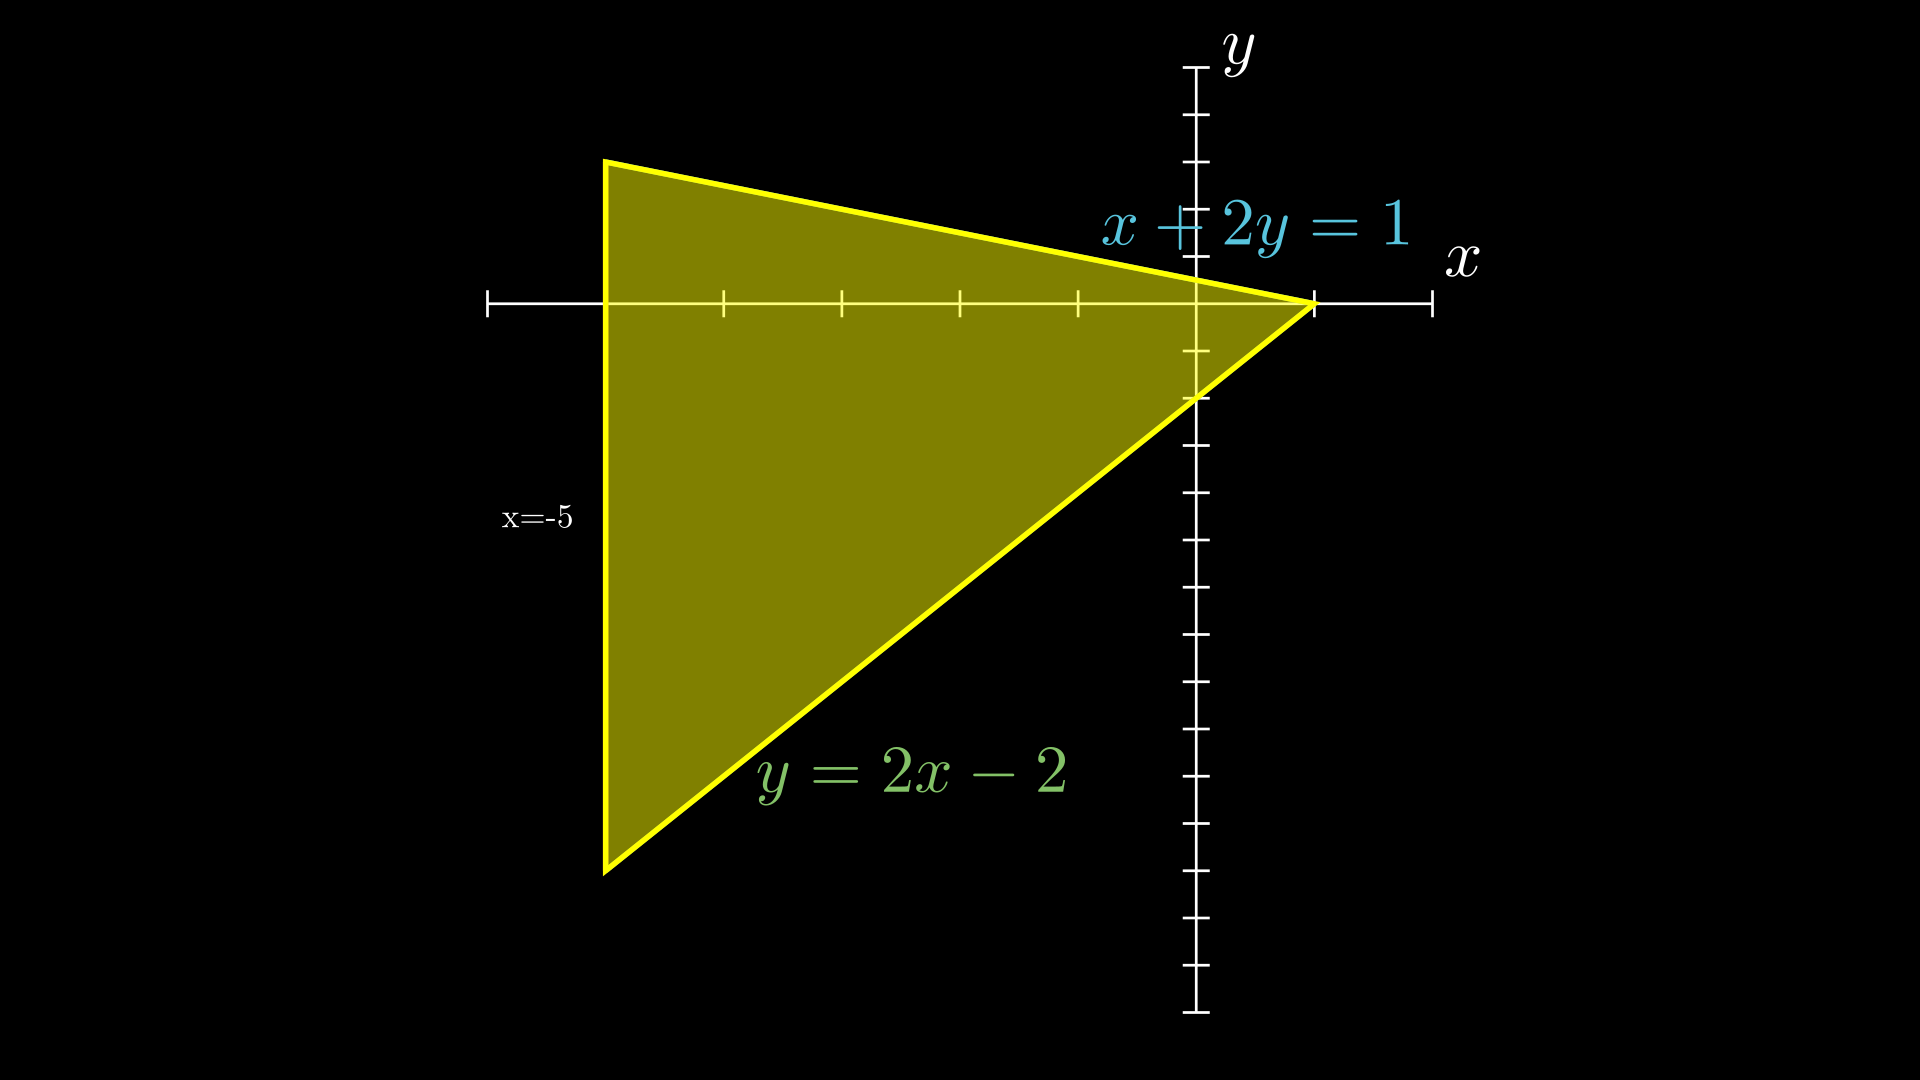
\includegraphics[width=0.8\linewidth]{SystemAScene.png}\\[0.5em]
    The feasible region is the triangle with vertices \((1,0)\), \((-5,3)\), and \((-5,-12)\).
    \item \textbf{Convex:} Yes.
    \item \textbf{Extreme Points:} \((1,0)\), \((-5,3)\), and \((-5,-12)\).
\end{itemize}

\subsection*{(b)}
We are given the inequalities
\[
x+y \ge 0,\quad x-y \le 0 \quad (\text{or } y\ge x),\quad x\ge 0.
\]

\subsubsection*{Calculations of the Extreme Point}
The constraints simplify to \(x\ge0\) and \(y\ge x\). Their boundaries intersect when:
\[
x=0 \quad \text{and} \quad y=x,
\]
which gives the point \((0,0)\). This is the only extreme point for this unbounded region.

\subsubsection*{Summary}
\begin{itemize}
    \item \textbf{Sketch:}\\[0.5em]
    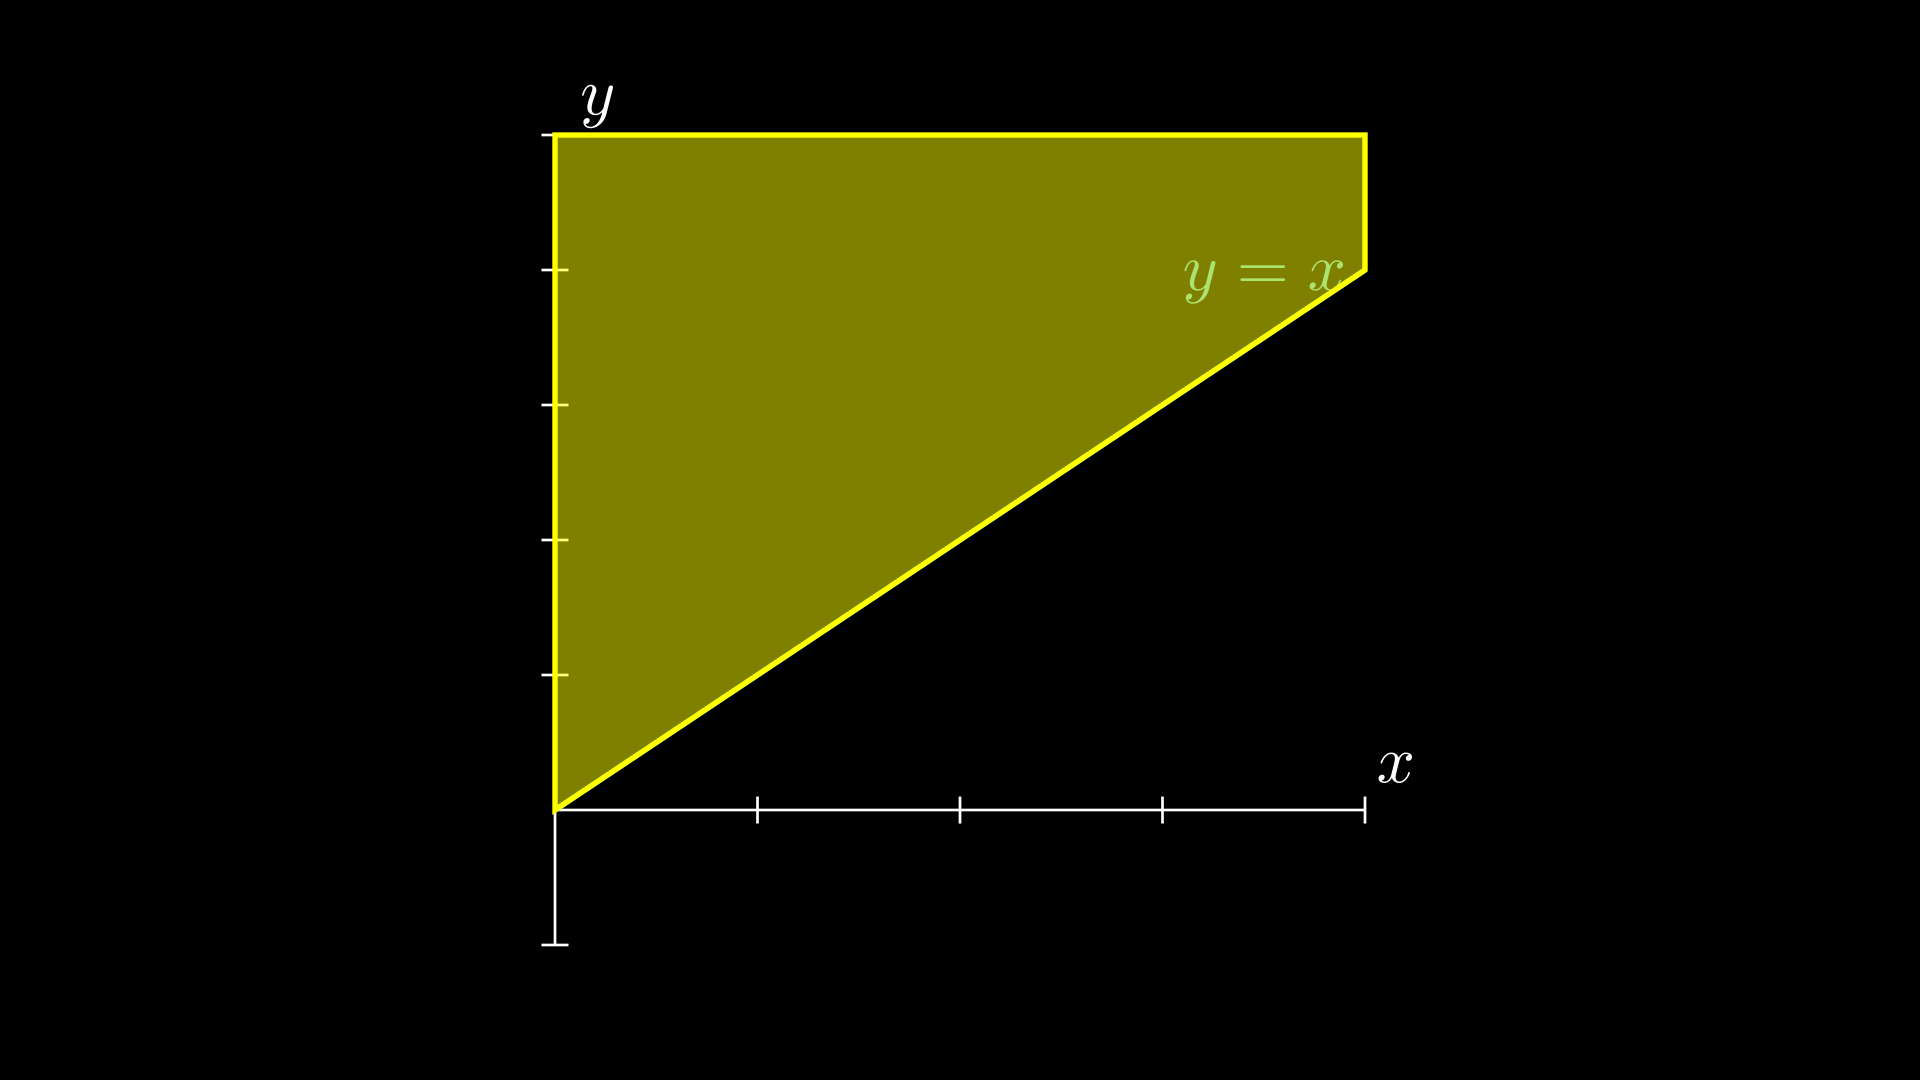
\includegraphics[width=0.8\linewidth]{SystemBScene.png}\\[0.5em]
    The region is the unbounded set defined by \(x\ge 0\) and \(y\ge x\); that is, the area in the first quadrant above (or on) the line \(y=x\).
    \item \textbf{Convex:} Yes.
    \item \textbf{Extreme Point:} \((0,0)\).
\end{itemize}

\subsection*{(c) (Bonus)}
We are given the inequalities
\[
x+y \ge 1,\quad x^2+y^2 \le 1.
\]

\subsubsection*{Calculations of Extreme Points}
\begin{enumerate}
    \item \textbf{Intersection of \(x+y=1\) and \(x^2+y^2=1\):}\\
    Express \(y=1-x\) and substitute into \(x^2+y^2=1\):
    \[
    x^2+(1-x)^2=1\quad\Longrightarrow\quad x^2+1-2x+x^2=1\quad\Longrightarrow\quad 2x^2-2x=0.
    \]
    Factor:
    \[
    2x(x-1)=0.
    \]
    Thus, \(x=0\) or \(x=1\). Then,
    \[
    \begin{cases}
    x=0 \quad \Rightarrow \quad y=1,\\[1mm]
    x=1 \quad \Rightarrow \quad y=0.
    \end{cases}
    \]
    Hence, the intersection points (the endpoints of the chord) are \((0,1)\) and \((1,0)\).
    
    \item \textbf{Other Extreme Points:}\\
    Since the unit disk \(x^2+y^2\le1\) is strictly convex, every point on the circular arc that satisfies \(x+y\ge1\) is an extreme point of the intersection. However, for the chord (the line segment between \((0,1)\) and \((1,0)\)), only the endpoints are extreme.
\end{enumerate}

\subsubsection*{Summary}
\begin{itemize}
    \item \textbf{Sketch:}\\[0.5em]
    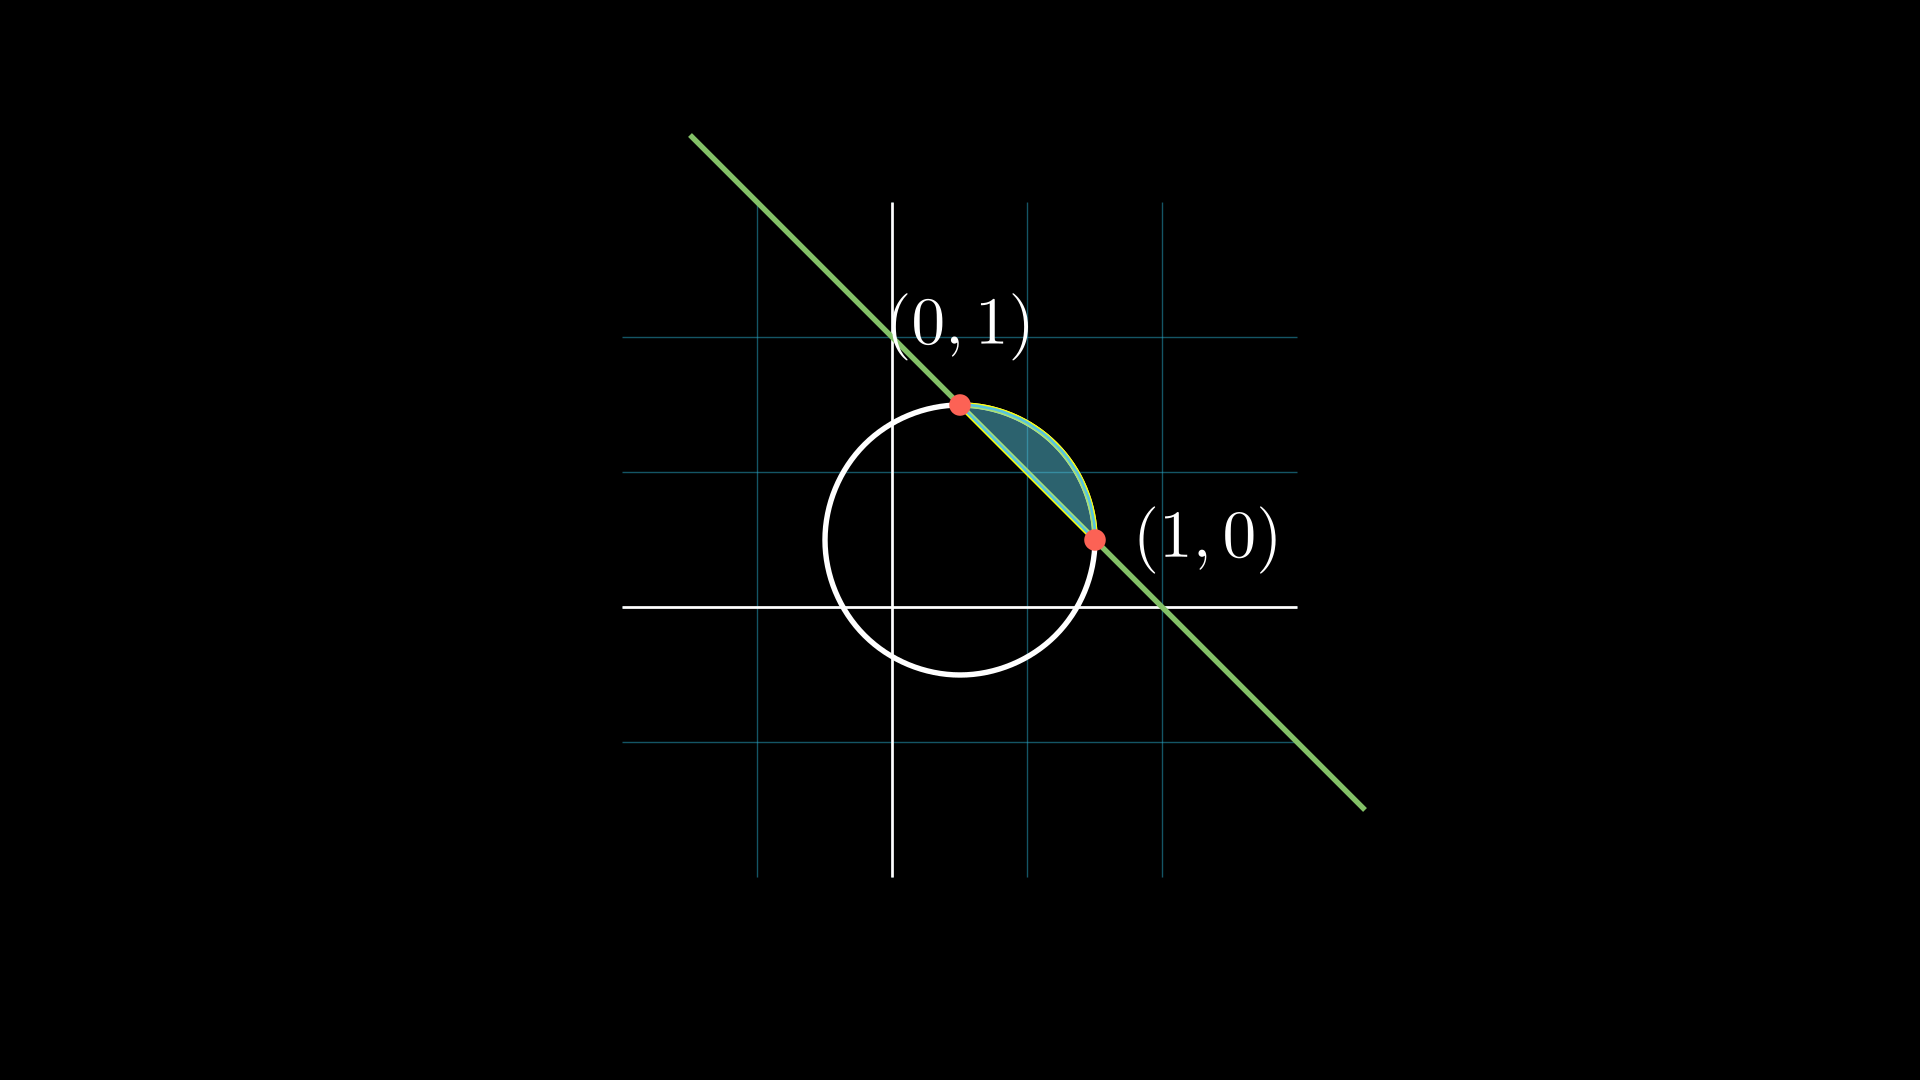
\includegraphics[width=0.8\linewidth]{SystemCScene.png}\\[0.5em]
    The region is the intersection of the unit disk \(x^2+y^2\le1\) and the half-plane \(x+y\ge1\), forming a circular segment (cap) with a boundary consisting of the circular arc from \((0,1)\) to \((1,0)\) and the chord joining these points.
    \item \textbf{Convex:} Yes.
    \item \textbf{Extreme Points:} The endpoints \((0,1)\) and \((1,0)\) and every point on the circular arc between them.
\end{itemize}


\section*{Question 5}

\subsection*{(a) Hyperplane in $\mathbb{R}^n$}

A \textbf{hyperplane} in $\mathbb{R}^n$ is defined as the set
\[
H = \{ x \in \mathbb{R}^n : a_1 x_1 + a_2 x_2 + \cdots + a_n x_n = b \},
\]
where the coefficient vector $a = (a_1, a_2, \dots, a_n)$ is nonzero and $b$ is a real number.

\medskip
\textbf{In $\mathbb{R}^2$:} The equation 
\[
x + y = 1
\]
represents a line (a 1-dimensional hyperplane in $\mathbb{R}^2$). This line intercepts the $x$–axis at $(1,0)$ and the $y$–axis at $(0,1)$.

\begin{figure}[H]
    \centering
    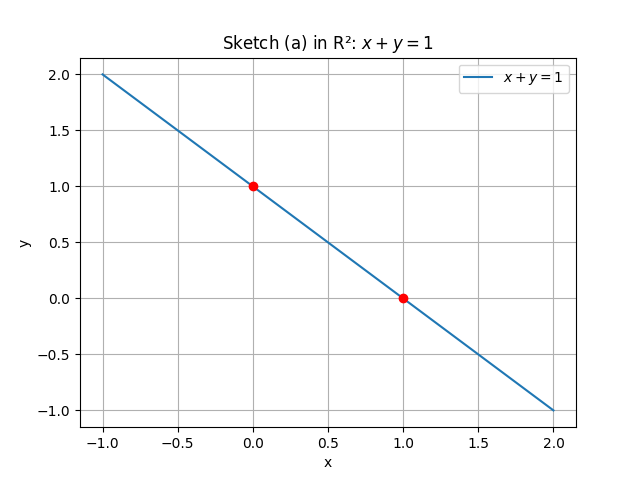
\includegraphics[width=0.5\textwidth]{a_R2.png}
    \caption{Sketch of $x+y=1$ in $\mathbb{R}^2$.}
\end{figure}

\medskip
\textbf{In $\mathbb{R}^3$:} The same equation, interpreted in $\mathbb{R}^3$, becomes
\[
\{(x,y,z) \in \mathbb{R}^3 : x+y=1\}.
\]
This is a plane (a 2-dimensional hyperplane in $\mathbb{R}^3$) that is ``vertical'' in the sense that the $z$-coordinate is free.

\begin{figure}[H]
    \centering
    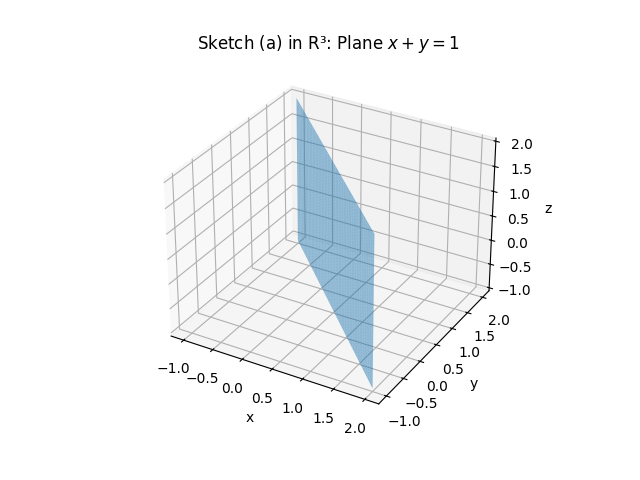
\includegraphics[width=0.5\textwidth]{a_R3.png}
    \caption{Sketch of the plane $x+y=1$ in $\mathbb{R}^3$.}
\end{figure}

\subsection*{(b) Half-Spaces Determined by a Hyperplane}

Given a hyperplane
\[
\{x \in \mathbb{R}^n : a^T x = b\},
\]
the two \textbf{half-spaces} are defined by the inequalities
\[
H^+ = \{x \in \mathbb{R}^n : a^T x \ge b\} \quad \text{and} \quad H^- = \{x \in \mathbb{R}^n : a^T x \le b\}.
\]

For the hyperplane 
\[
2x + y = 4
\]
in $\mathbb{R}^2$, the two half-spaces are
\[
H^+ = \{(x,y) : 2x+y \ge 4\} \quad \text{and} \quad H^- = \{(x,y) : 2x+y \le 4\}.
\]

\medskip
\textbf{Sketch (Half-spaces):}
\begin{figure}[H]
    \centering
    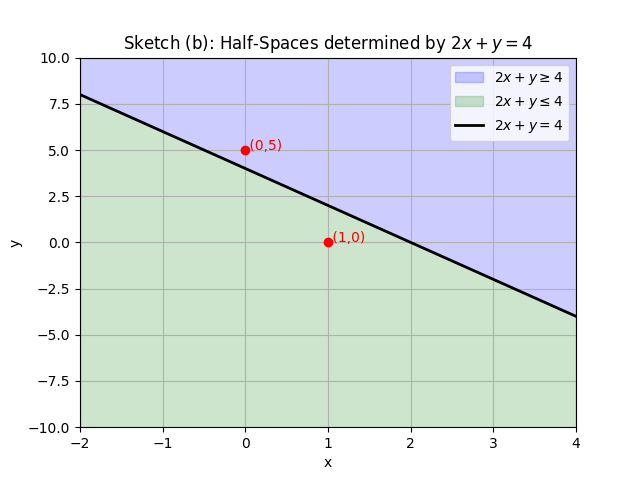
\includegraphics[width=0.5\textwidth]{b.png}
    \caption{Half-spaces determined by $2x+y=4$. The point $(1,0)$ lies in $H^-$ and $(0,5)$ in $H^+$.}
\end{figure}

For the point $(1,0)$:
\[
2(1)+0 = 2 < 4 \quad \Rightarrow \quad (1,0) \in H^-.
\]
For the point $(0,5)$:
\[
2(0)+5 = 5 > 4 \quad \Rightarrow \quad (0,5) \in H^+.
\]
Since these points lie in different half-spaces, the line $2x+y=4$ \textbf{does} separate them.

\subsection*{(c) Hyperplane Separating Two Sets}

A hyperplane $H$ is said to \textbf{separate} two sets $A$ and $B$ if
\[
A \subset H^- \quad \text{and} \quad B \subset H^+ \quad \text{(or vice versa)}
\]
and neither set crosses $H$.

The given sets in $\mathbb{R}^2$ are:
\begin{itemize}
    \item $A = \{(x,y) \in \mathbb{R}^2 : x^2+y^2 \le \tfrac{1}{4}\}$, a closed disk centered at $(0,0)$ with radius $\tfrac{1}{2}$.
    \item $B = \{(x,y) \in \mathbb{R}^2 : (x-2)^2+(y-2)^2 \le \tfrac{1}{4}\}$, a closed disk centered at $(2,2)$ with radius $\tfrac{1}{2}$.
\end{itemize}

\medskip
\textbf{Checking their positions relative to $2x+y=4$:}

For the center of $A$, $(0,0)$:
\[
2(0)+0 = 0 < 4.
\]
The distance from $(0,0)$ to the line is 
\[
\frac{|0-4|}{\sqrt{2^2+1^2}} = \frac{4}{\sqrt{5}} \approx 1.788,
\]
which is greater than $\tfrac{1}{2}$. Thus, the entire disk $A$ lies in the half-space $2x+y<4$.

For the center of $B$, $(2,2)$:
\[
2(2)+2 = 6 > 4.
\]
The distance from $(2,2)$ to the line is
\[
\frac{|6-4|}{\sqrt{5}} = \frac{2}{\sqrt{5}} \approx 0.894,
\]
which is also greater than $\tfrac{1}{2}$. Thus, the entire disk $B$ lies in the half-space $2x+y>4$.

\begin{figure}[H]
    \centering
    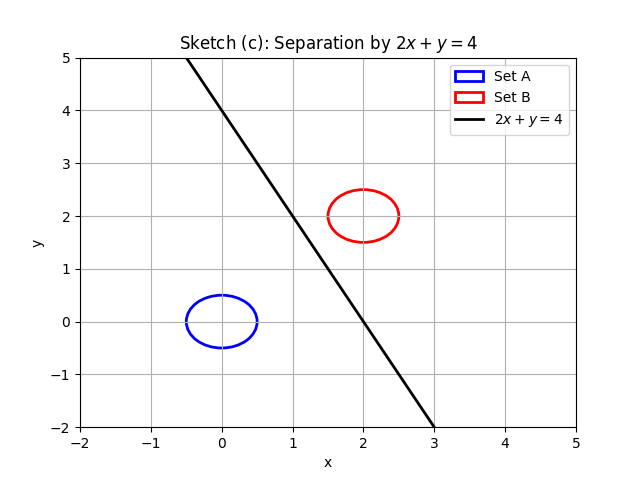
\includegraphics[width=0.5\textwidth]{c.png}
    \caption{Separation of the disks by the line $2x+y=4$.}
\end{figure}

Since neither disk intersects the line and each lies completely in a different half-space, the line $2x+y=4$ \textbf{separates} the two sets.

\subsection*{(d) Separating Hyperplane Theorem and Convexity}

The \textbf{separating hyperplane theorem} states that if $A$ and $B$ are two nonempty, disjoint, \textbf{convex} subsets of $\mathbb{R}^n$, then there exists a hyperplane that separates them.

\medskip
\textbf{Question:} Can we remove the condition of ``convex sets''?\\[5pt]
\textbf{Answer:} \textbf{No.}

\medskip
\textbf{Reason:} Convexity is crucial. If one (or both) of the sets is nonconvex, even if they are disjoint, there might be no single hyperplane that can separate them.

\medskip
\textbf{Counterexample:} Consider in $\mathbb{R}^2$ the following sets:
\begin{itemize}
    \item $A = \{(x,\sin(1/x)) : x \in (0,1]\} \cup \{(0,0)\}$ (nonconvex because of its oscillatory behavior as $x \to 0^+$).
    \item $B = \{(x,0) : x \in [0,1]\}$, which is convex.
\end{itemize}
Although $A$ and $B$ are disjoint, the rapid oscillations of $A$ near $x=0$ prevent any straight line (hyperplane in $\mathbb{R}^2$) from lying entirely between them.

\subsection*{(e) Supporting and Tangential Hyperplanes}

\textbf{Supporting Hyperplane:} A hyperplane $H$ is a \textbf{supporting hyperplane} of a set $S$ if 
\begin{enumerate}
    \item $H$ intersects $S$ (i.e., $H \cap S \neq \varnothing$), and 
    \item $S$ lies entirely in one of the closed half-spaces determined by $H$.
\end{enumerate}

\medskip
\textbf{Tangential Hyperplane:} A \textbf{tangential hyperplane} is a supporting hyperplane that ``just touches'' the set $S$ at a boundary point (or along a boundary curve) without cutting through its interior. In classical calculus, a tangent line to a smooth curve is a tangential hyperplane in $\mathbb{R}^2$.

\medskip
\textbf{Examples in $\mathbb{R}^2$:}

\medskip
\textbf{1. Tangential Hyperplane Example:}  
Let 
\[
S = \{(x,y) \in \mathbb{R}^2 : x^2+y^2 \le 1\} \quad \text{(the unit disk)}.
\]
The line 
\[
x = 1
\]
touches $S$ only at the point $(1,0)$ and $S$ lies entirely in $\{x \le 1\}$. Hence, $x=1$ is a tangential hyperplane.

\begin{figure}[H]
    \centering
    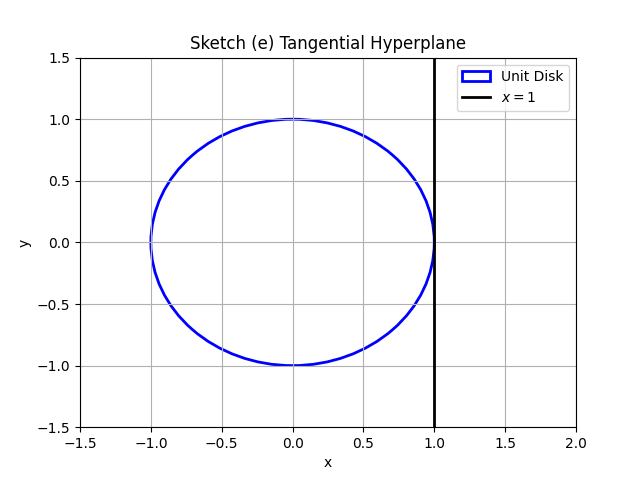
\includegraphics[width=0.5\textwidth]{e_tangent.png}
    \caption{Tangential hyperplane: $x=1$ touching the unit disk.}
\end{figure}

\medskip
\textbf{2. Supporting (but not Tangential) Hyperplane Example:}  
Consider the square
\[
S = \{(x,y) \in \mathbb{R}^2 : 0 \le x \le 1,\; 0 \le y \le 1\}.
\]
The line 
\[
x = 1
\]
is a supporting hyperplane since $S \subset \{x \le 1\}$ and the hyperplane meets $S$ along the entire vertical edge $\{1\} \times [0,1]$.

\begin{figure}[H]
    \centering
    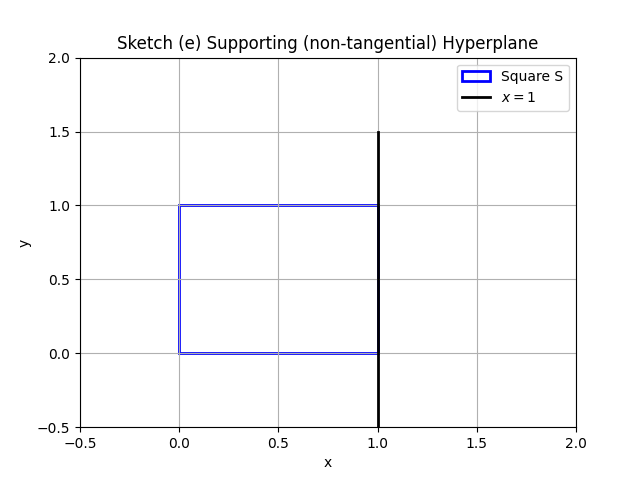
\includegraphics[width=0.5\textwidth]{e_supporting.png}
    \caption{Supporting (non-tangential) hyperplane: $x=1$ supporting the square.}
\end{figure}

\subsection*{(f) Extreme Points of a Set}

An \textbf{extreme point} of a convex set $S$ is a point $x \in S$ that cannot be written as a convex combination
\[
x = t\,y + (1-t)\,z, \quad 0 < t < 1,
\]
of two distinct points $y, z \in S$.

Consider the set
\[
S = \{ (x,y) \in \mathbb{R}^2 : x \in [0,\pi],\; y \le \sin(x) \}.
\]
This is the region in $\mathbb{R}^2$ that lies below (or on) the curve $y=\sin(x)$ for $x \in [0,\pi]$.

The \textbf{upper boundary} of $S$ is given by the graph
\[
\{ (x, \sin(x)) : x \in [0,\pi] \}.
\]
Since $\sin(x)$ is strictly concave on $(0,\pi)$ (because $\sin''(x) = -\sin(x) < 0$ for $x\in(0,\pi)$), every point on the curve is exposed to the top and cannot be expressed as a convex combination of other points in $S$. In particular, the endpoints $(0,0)$ and $(\pi,0)$ are extreme.

\begin{figure}[H]
    \centering
    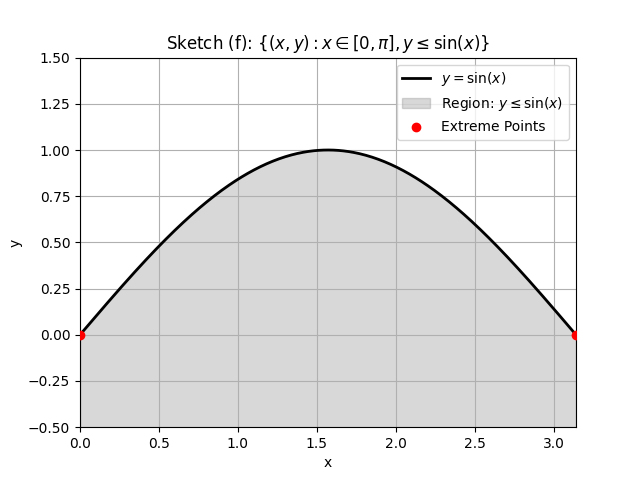
\includegraphics[width=0.5\textwidth]{f.png}
    \caption{Sketch of the set $S = \{(x,y): x\in[0,\pi],\, y \le \sin(x)\}$, showing the curve $y=\sin(x)$ and extreme points at $(0,0)$ and $(\pi,0)$.}
\end{figure}

\end{document}